\newcommand{\deadline}{14.07.2023}

\documentclass[11pt]{article}

\usepackage[exercise,ex]{custom_2.1}

\begin{document}

\section{Plattenkondensator mit Dielektrikum}
\subsection{}
\begin{align*}
    E_L &= \frac{U_L}{d_L}\\
    &= 2\epsilon_r \frac{U_P}{d_P}\\
    &= 2\epsilon_r E_P\\
    \frac{E_P}{E_L} &= \frac{1}{2\epsilon_r}\\
    &\approx 0.278\\
\end{align*}

\subsection{}
\begin{align*}
    U &= 2U_L + U_P\\
    &= 2U_L + \frac{U_L}{\epsilon_r}\\
    U_L &= \frac{U}{{2+ \frac1{\epsilon_r}}}\\
    E_L &=  \frac{U}{d}\frac{1}{{2+ \frac1{\epsilon_r}}}\\
    &\approx \frac{600 \u V}{5\u{mm}}\frac{1}{2+ \frac{1}{1.8}}\\
    &\approx 93.9 \ufrac {kV}m\\
    \\
    U_P &= \frac{1}{\epsilon_r}\frac{U}{{2+ \frac1{\epsilon_r}}}\\
    E_P &= \frac{1}{\epsilon_r d_P}\frac{U}{{2+ \frac1{\epsilon_r}}}\\
    &\approx \frac{1}{1.8\cdot 5\u {mm}}\frac{600 \u V}{2+ \frac{1}{1.8}}\\
    &\approx 26.1 \ufrac{kV}{m}
\end{align*}

\subsection{}
\begin{align*}
\end{align*}

\subsection{}
\begin{align*}
    \frac1C &=\frac{2}{C_L} + \frac{1}{C_P}\\
    &= \frac{2d_L}{\epsilon_0 A} + \frac{d_P}{\epsilon_0\epsilon_r A}\\
    &= \frac{2d_L}{\epsilon_0 A}\hug{1+ \frac{1}{\epsilon_r}}\\
    C &= \frac{\epsilon_0 A}{2d_L}\frac{1}{1 + \frac{1}{\epsilon_r}}\\
    &\approx \frac{\epsnull\cdot 200\u{cm^2}}{2\cdot 2.5\u{mm}} \frac{1}{1 + \frac{1}{1.8}}\\
    &\approx 22.8 \u{pF} \\
    \\
    C &= \frac{Q}{U}\\
    Q &= CU\\
    &= \frac{\epsilon_0 A U}{2d}\frac{1}{1 + \frac{1}{\epsilon_r}}\\
    &= \frac{\epsnull\cdot 200\u{cm^2}\cdot 600 \u V}{2\cdot 5\u{mm}} \frac{1}{1 + \frac{1}{1.8}}\\
    &\approx 6.84\u{nC}
\end{align*}

\subsection{}
\begin{align*}
    \frac{W_P}{W} &=  \frac{C_P U_P^2}{C U^2}\\
    \\
    \frac{C_P}C &=\frac{2C_P}{C_L} + 1\notethat[siehe (b)]\\
    &= \epsilon_r+1\\
    \\
    U_P &= \frac{1}{\epsilon_r}\frac{U}{{2+ \frac1{\epsilon_r}}}\notethat[siehe (b)]\\
    \frac{U_P}U &= \frac{1}{2\epsilon_r+ 1}\\
    \\
    \frac{W_P}{W} &=  \frac{C_P U_P^2}{C U^2}\\
    &= \frac{\epsilon_r+1}{\hug{2\epsilon_r+ 1}^2}\\
    &\approx \frac{1.8+1}{\hug{2\cdot1.8+ 1}^2}\\
    &\approx 13.2 \%
\end{align*}

\subsection{}
\begin{align*}
    W &= \frac{1}{2}CU^2\\
    &\approx \frac{1}{2} \cdot 6.84\u{nC} \cdot 600^2\u V^2\\
    &\approx 4.11\u{\micro J}
\end{align*}

\section{Poynting-Vektor}
\subsection{}
\begin{figure}[h]
    \centering
    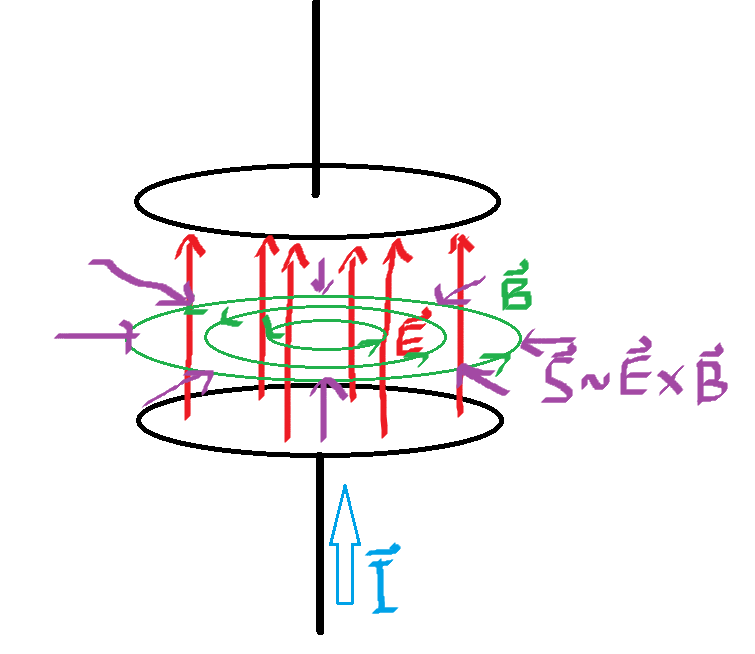
\includegraphics[width=0.5\textwidth]{F1.png}
    \begin{adjustwidth}{20pt}{}
        \caption{Poynting Vektoren bei Aufladen eines kreisförmigen Plattenkondensators.
        (Tatsächlich würden sich die B-Felder bei einem perfekt homogenen Feld 
        im Inneren des Kondensators gegenseitig wegheben, deswegen die 
        beiden inneren B-Feldlinien bitte einfach ignorieren)}
    \end{adjustwidth}
\end{figure}

\subsection{}
\begin{adjustwidth}{20pt}{}
    Der Poynting-Vektors zeigt, wie man in der Skizze gut nachvollziehen kann, 
    radial nach innen.
\end{adjustwidth}
\begin{align*}
    0 &= U + U_R + U_C\\
    &= U + R I + \frac{Q}{C}\\
    &= U + R \dot Q + \frac{Q}{C}\\
    \dot Q &= - \frac{Q}{RC} - \frac{U}{R}\\
    Q(t) &= c\cdot e^{-\frac{t}{RC}} - UC \notethat c\in\R\\
    Q(0) &= 0 \implies Q(t) = UC \hug{e^{-\frac{t}{RC}} - 1} \\
    \\
    \vec S (t)&=  \epsilon_0 c^2 (\vec E (t)\times \vec B(t))\\
    \sabs{\vec S}(t) &=  \epsilon_0 c^2 \sabs{\vec E}\cdot\sabs{\vec B}\\
    &= \epsilon_0 c E^2\\
    &= \epsilon_0 c \frac{U^2}{d^2}\\
    &= \epsilon_0 c \frac{Q^2}{d^2 C^2}\\
    &= \epsilon_0 c \frac{U^2C^2 \hug{e^{-\frac{t}{RC}} - 1}^2}{d^2 C^2}\\
    &= \epsilon_0 c \frac{U^2}{d^2} \hug{e^{-\frac{t}{RC}} - 1}^2\\
    &= \epsilon_0 c E_{max}^2 \hug{e^{-\frac{t}{RC}} - 1}^2\\
    &= I_{max} \hug{e^{-\frac{t}{RC}} - 1}^2\notethat I\equiv\te{Intensität}\\
\end{align*}

\subsection{}
\begin{align*}
\end{align*}

\subsection{}
\begin{align*}
\end{align*}

\section{Dipolstrahlung}
\subsection{}
\begin{align*}
    c &= I(\theta,r)\notethat c\in\R  \te{ beliebig aber fest}\\
    &= \frac{\omega^4 P_0^2}{2(4\pi)^2\epsilon_0 c^3}\cdot \frac{\sin^2(\theta)}{r^2}\\
    c &= \frac{\sin^2(\theta)}{r^2}\\
    c &= \frac{\sin(\theta)}{r}\\
    r &= c \sin(\theta)\
\end{align*}
\begin{adjustwidth}{20pt}{}
    Letzteres ist die bekannte Vorschrift für einen den Ursprung tangierenden Kreis in 
    Polarkoordinaten mit Radius \(r=\frac{c}{2}\) . 
\end{adjustwidth}

\subsection{}
\begin{align*}
    I_{ges} &= \int_{\mathcal S} I(\theta,r)\dS\\
    &= \int_{0}^{2\pi}\negspace\dphi\int_{0}^{\pi}\hspace{-0.2cm}\dtheta I(\theta,r)\cdot r^2 \sin\theta\\
    &= 2\pi\cdot \frac{1}{2}\frac{\omega^4 P_0^2}{(4\pi)^2 \epsilon_0 c^3}\int_{0}^{\pi}\hspace{-0.2cm}\dtheta \frac{\sin^2\theta}{r^2}\cdot r^2 \sin\theta\\
    &= \underbrace{\frac{\omega^4 P_0^2}{16\pi^2 \epsilon_0 c^3}}_{\eta}\int_{0}^{\pi}\hspace{-0.2cm}\dtheta\sin^3\theta\\
    &= \frac \eta2 \int_{0}^{\pi}\hspace{-0.2cm}\dtheta(\sin\theta-\cos(2\theta)\sin\theta)\\
    &= \eta - \frac\eta2\int_{0}^{\pi}\hspace{-0.2cm}\dtheta\cos(2\theta)\sin\theta\\
    &= \eta - \frac\eta4 \int_{0}^{\pi}\hspace{-0.2cm}\dtheta\hug{\sin(3\theta)-\sin\theta}\\
    &= \eta + \frac\eta2- \frac\eta4 \int_{0}^{\pi}\hspace{-0.2cm}\dtheta\hug{\sin(3\theta)}\\
    &= \eta + \frac\eta2 + \frac\eta{12} \cos(3\theta)\eval_{0}^{\pi}\\
    &= \eta + \frac\eta2 - \frac\eta{6}\\
    &= \frac{4}{3}\eta\\
    &= \frac{\omega^4 P_0^2}{12\pi^2 \epsilon_0 c^3}\\
\end{align*}

\end{document}